% This is samplepaper.tex, a sample chapter demonstrating the
% LLNCS macro package for Springer Computer Science proceedings;
% Version 2.21 of 2022/01/12
%
\documentclass[runningheads]{llncs}
%
\usepackage[T1]{fontenc}
% T1 fonts will be used to generate the final print and online PDFs,
% so please use T1 fonts in your manuscript whenever possible.
% Other font encondings may result in incorrect characters.
%
\usepackage{graphicx}
% Used for displaying a sample figure. If possible, figure files should
% be included in EPS format.
%
% If you use the hyperref package, please uncomment the following two lines
% to display URLs in blue roman font according to Springer's eBook style:
%\usepackage{color}
%\renewcommand\UrlFont{\color{blue}\rmfamily}
%\urlstyle{rm}
%
\begin{document}
%
\title{Contribution Title}
%
%\titlerunning{Abbreviated paper title}
% If the paper title is too long for the running head, you can set
% an abbreviated paper title here
%
\author{Rodrigo Prestes Machado\inst{1}\orcidID{0000-0003-0428-6387} \and
Second Author\inst{2,3}\orcidID{1111-2222-3333-4444} \and
Third Author\inst{3}\orcidID{2222--3333-4444-5555}}
%
\authorrunning{F. Author et al.}
% First names are abbreviated in the running head.
% If there are more than two authors, 'et al.' is used.
%
\institute{Princeton University, Princeton NJ 08544, USA \and
Springer Heidelberg, Tiergartenstr. 17, 69121 Heidelberg, Germany
\email{lncs@springer.com}\\
\url{http://www.springer.com/gp/computer-science/lncs} \and
ABC Institute, Rupert-Karls-University Heidelberg, Heidelberg, Germany\\
\email{\{abc,lncs\}@uni-heidelberg.de}}
%
\maketitle              % typeset the header of the contribution
%
\begin{abstract}
The aim of this study is to analyze the interactions of programming students
with a chatbot powered by OpenAI's GPT-3.5, enhanced with the Retrieval
Augmented Generation (RAG) technique, within the context of a Java programming
course. The study investigates how students use the chatbot while employing
two metacognitive strategies: interleaving and spacing. The methodology involved
classifying and categorizing the students' interaction prompts with the chatbot
into eight distinct categories. The findings reveal that, while most
interactions focus on active learning strategies, students demonstrate limited
conscious application of metacognitive strategies. The study highlights the need
for more comprehensive guidance on the strategic use of AI tools to enhance
learning outcomes.

\keywords{Programming \and Generative Artificial Intelligence \and Chatbots \and
Spacing \and Interleaving \and Metacognition.}
\end{abstract}
%
%
%
\section{Theoretical Framework}
\subsection{Metacognition}
Given that GenAI often produces highly accurate and automatic responses
\cite{Puryear22}, it is essential that students use these tools within an
active learning process to enhance their learning outcomes. This active
learning process can be further understood through the lens of metacognition,
which focuses on awareness of one's mental processes. \cite{flavell79}
proposed a model of metacognitive monitoring that includes four interrelated
phenomena: Metacognitive Knowledge, Metacognitive Experience, Metacognitive
Goals, and Metacognitive Actions. These processes do not occur in isolation, but
they influence each other, altering cognitive progress over time.

Metacognitive knowledge includes beliefs about variables that affect the
outcomes of cognitive activities. It is divided into three types: beliefs about
personal abilities, perceived difficulty in the task, and previously used
strategies. Metacognitive Experience refers to the feelings that arise before,
during, and after cognitive activity, such as frustration, confusion,
satisfaction, and others. Metacognitive Goals are the key to regulating thought
as they relate to the goals the individual seeks to achieve, directly
influencing the actions taken. For example, if a student’s goal is to complete
a task quickly, they may adopt a more passive approach to learning. Lastly,
Metacognitive Actions involve the planning, monitoring, and evaluation of
strategies used to achieve the goals. In terms of planning, students can
determine how to approach a task, such as spacing their study sessions
\cite{Ouhao18,Carvalho20} interleaving topics \cite{Rivers21}, utilizing
retrieval practice \cite{larsen18}, and other possible strategies.

Spacing and interleaving are two metacognitive strategies that have been shown
to enhance learning outcomes and support the research questions of this study.
Spacing refers to the practice of distributing study sessions over time, which
has been shown to improve long-term retention and understanding of the material
\cite{Carvalho20}. Interleaving involves mixing different topics or problems
within a single learning session, which has been shown to also enhance long-term
learning and the application of student's knowledge in other contexts and
situations \cite{Rivers21}.


\subsubsection{Sample Heading (Third Level)} Only two levels of
headings should be numbered. Lower level headings remain unnumbered;
they are formatted as run-in headings.

\paragraph{Sample Heading (Fourth Level)}
The contribution should contain no more than four levels of
headings. Table~\ref{tab1} gives a summary of all heading levels.

\begin{table}
\caption{Table captions should be placed above the
tables.}\label{tab1}
\begin{tabular}{|l|l|l|}
\hline
Heading level &  Example & Font size and style\\
\hline
Title (centered) &  {\Large\bfseries Lecture Notes} & 14 point, bold\\
1st-level heading &  {\large\bfseries 1 Introduction} & 12 point, bold\\
2nd-level heading & {\bfseries 2.1 Printing Area} & 10 point, bold\\
3rd-level heading & {\bfseries Run-in Heading in Bold.} Text follows & 10 point, bold\\
4th-level heading & {\itshape Lowest Level Heading.} Text follows & 10 point, italic\\
\hline
\end{tabular}
\end{table}


\noindent Displayed equations are centered and set on a separate
line.
\begin{equation}
x + y = z
\end{equation}
Please try to avoid rasterized images for line-art diagrams and
schemas. Whenever possible, use vector graphics instead (see
Fig.~\ref{fig1}).

\begin{figure}
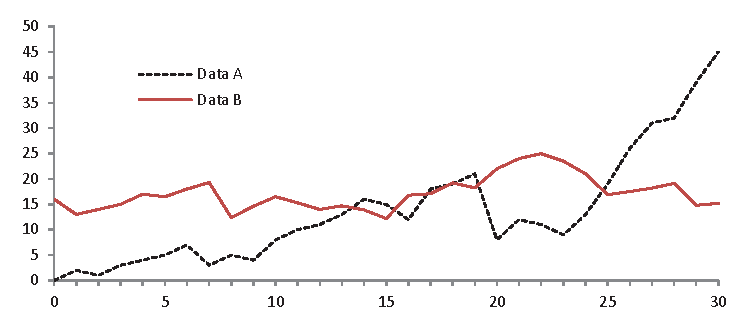
\includegraphics[width=\textwidth]{fig1.eps}
\caption{A figure caption is always placed below the illustration.
Please note that short captions are centered, while long ones are
justified by the macro package automatically.} \label{fig1}
\end{figure}

\begin{theorem}
This is a sample theorem. The run-in heading is set in bold, while
the following text appears in italics. Definitions, lemmas,
propositions, and corollaries are styled the same way.
\end{theorem}
%
% the environments 'definition', 'lemma', 'proposition', 'corollary',
% 'remark', and 'example' are defined in the LLNCS documentclass as well.
%
\begin{proof}
Proofs, examples, and remarks have the initial word in italics,
while the following text appears in normal font.
\end{proof}
For citations of references, we prefer the use of square brackets
and consecutive numbers. Citations using labels or the author/year
convention are also acceptable. The following bibliography provides
a sample reference list with entries for journal
articles~\cite{ref_article1}, an LNCS chapter~\cite{ref_lncs1}, a
book~\cite{ref_book1}, proceedings without editors~\cite{ref_proc1},
and a homepage~\cite{ref_url1}. Multiple citations are grouped
\cite{ref_article1,ref_lncs1,ref_book1},
\cite{ref_article1,ref_book1,ref_proc1,ref_url1}.

\begin{credits}
\subsubsection{\ackname} A bold run-in heading in small font size at the end of the paper is
used for general acknowledgments, for example: This study was funded
by X (grant number Y).

\subsubsection{\discintname}
It is now necessary to declare any competing interests or to specifically
state that the authors have no competing interests. Please place the
statement with a bold run-in heading in small font size beneath the
(optional) acknowledgments\footnote{If EquinOCS, our proceedings submission
system, is used, then the disclaimer can be provided directly in the system.},
for example: The authors have no competing interests to declare that are
relevant to the content of this article. Or: Author A has received research
grants from Company W. Author B has received a speaker honorarium from
Company X and owns stock in Company Y. Author C is a member of committee Z.
\end{credits}
%
% ---- Bibliography ----
%
% BibTeX users should specify bibliography style 'splncs04'.
% References will then be sorted and formatted in the correct style.
%
\bibliographystyle{splncs04}
\bibliography{References}
\end{document}